\newcommand{\guishot}[2]{% {檔名}{說明}
\begin{figure}[htbp]\centering\includegraphics[width=0.92\linewidth]{img/#1}\caption{#2}\end{figure}}

同一個網站依登入者的角色顯示三種介面：顧客購物介面、工作人員管理介面與平台管理介面。以下截圖為系統以 4.7 節的示範資料啟動後實際操作的畫面。

\subsubsection*{顧客購物介面}

未登入的訪客也可以瀏覽商品。首頁（圖 \ref{fig:gui_home}）上方列出今天有效的折扣政策，可以依關鍵字、商店與類別搜尋商品；點選商品進入商品頁（圖 \ref{fig:gui_product}）。商店一覽（圖 \ref{fig:gui_stores}）列出三間商店與其平均評分。

\guishot{gui_home.png}{\label{fig:gui_home}首頁：今日優惠、商品搜尋與篩選}
\guishot{gui_product.png}{\label{fig:gui_product}商品頁}
\guishot{gui_stores.png}{\label{fig:gui_stores}商店一覽與評分}

登入頁（圖 \ref{fig:gui_login}）以帳號與密碼登入，已停用的帳號無法登入。顧客登入後可以把商品加入購物車並調整數量（圖 \ref{fig:gui_cart}），結帳後在「我的訂單」查看所有訂單與消費總額（圖 \ref{fig:gui_my_orders}）；訂單詳情顯示訂單進度與狀態歷程（圖 \ref{fig:gui_order_detail}），狀態歷程即 \at{order_status_history} 中由 trigger 寫入的資料。

\guishot{gui_login.png}{\label{fig:gui_login}登入頁}
\guishot{gui_cart.png}{\label{fig:gui_cart}購物車（顧客 alice）}
\guishot{gui_my_orders.png}{\label{fig:gui_my_orders}我的訂單}
\guishot{gui_order_detail.png}{\label{fig:gui_order_detail}訂單詳情與狀態歷程（訂單 \#5）}

\subsubsection*{工作人員管理介面}

工作人員登入後進入後台總覽（圖 \ref{fig:gui_staff_dashboard}），顯示期間內的訂單數、銷售總額、各狀態的訂單數與待審核的退貨。商品與庫存（圖 \ref{fig:gui_staff_products}）可以新增、修改、上下架與刪除商品；已被訂單引用的商品刪除時會改為下架（BR-20）。

\guishot{gui_staff_dashboard.png}{\label{fig:gui_staff_dashboard}工作人員後台總覽}
\guishot{gui_staff_products.png}{\label{fig:gui_staff_products}商品與庫存管理}

隸屬商店的工作人員只能管理自己商店的資料（BR-21）。圖 \ref{fig:gui_store_staff_products} 是台北信義店店員 \texttt{staff\_xinyi} 登入後的商品頁，商店篩選固定為自己的商店，只列出該店的 5 項商品；訂單、退貨與報表也只顯示含該店商品的資料。

\guishot{gui_store_staff_products.png}{\label{fig:gui_store_staff_products}商店工作人員只看得到自己商店的商品}

訂單管理（圖 \ref{fig:gui_staff_orders}）可以依狀態、日期與關鍵字查詢訂單；在訂單詳情（圖 \ref{fig:gui_staff_order_detail}）依 BR-19 的順序推進狀態。圖中訂單 \#10 有待審核的退貨申請，因此依 BR-25 不能推進狀態，畫面上方顯示提示。

\guishot{gui_staff_orders.png}{\label{fig:gui_staff_orders}訂單管理}
\guishot{gui_staff_order_detail.png}{\label{fig:gui_staff_order_detail}訂單詳情：有待審核退貨時不能推進狀態（BR-25）}

退貨審核（圖 \ref{fig:gui_staff_returns}）列出所有退貨申請，核准時依 BR-26 計算退款金額。折扣管理（圖 \ref{fig:gui_staff_discounts}）管理特殊活動、季節性與運費三種折扣，特殊活動折扣可以指定適用商品，期間重疊時會被 5.4 節的 BR-13 trigger 拒絕。銷售報表（圖 \ref{fig:gui_staff_reports}）依日、週、月統計各商店的銷售額，計算方式與 Section 8 的檢視表 V1 相同（BR-23）。

\guishot{gui_staff_returns.png}{\label{fig:gui_staff_returns}退貨審核}
\guishot{gui_staff_discounts.png}{\label{fig:gui_staff_discounts}折扣管理}
\guishot{gui_staff_reports.png}{\label{fig:gui_staff_reports}銷售報表}

\subsubsection*{平台管理介面}

平台管理員可以查詢、新增與修改使用者帳號，指派角色、指定工作人員所屬的商店（未指定即為總部人員，AAS-F-009），以及停用或啟用任何帳號（圖 \ref{fig:gui_admin_users}）；系統至少保留一位啟用中的平台管理員。商店資料（圖 \ref{fig:gui_admin_stores}）用來新增商店（STS-F-005）與修改各商店的聯絡資訊（STS-F-002）。

\guishot{gui_admin_users.png}{\label{fig:gui_admin_users}使用者帳號、角色與停用／啟用}
\guishot{gui_admin_stores.png}{\label{fig:gui_admin_stores}商店資料}

\subsubsection*{手機版}

網站採用響應式版面，在手機寬度下導覽列收成選單按鈕，商品列表改為兩欄，後台側欄也會收合（圖 \ref{fig:gui_mobile}）。

\begin{figure}[htbp]\centering
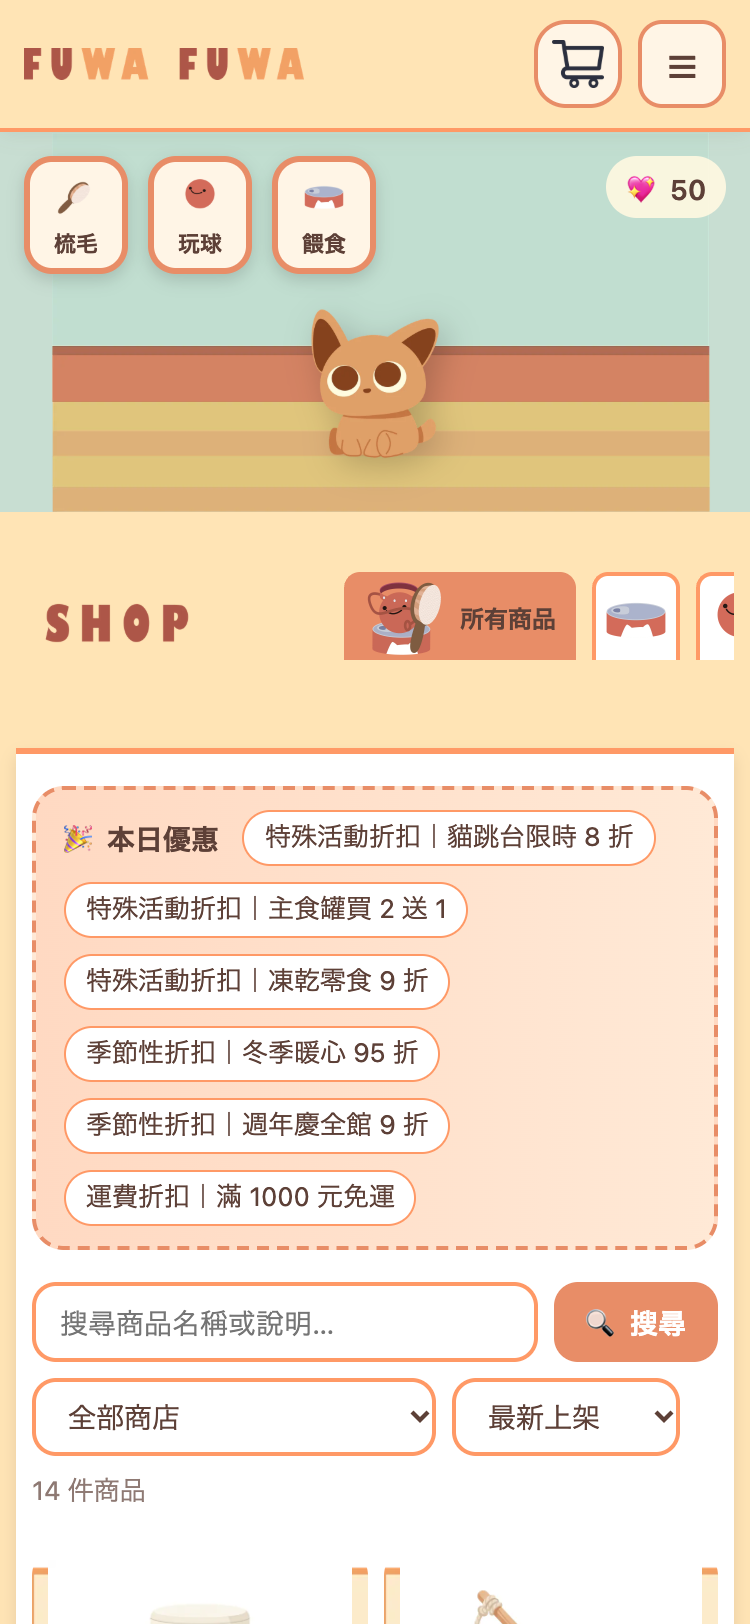
\includegraphics[width=0.36\linewidth]{img/gui_mobile_home.png}\hspace{2em}%
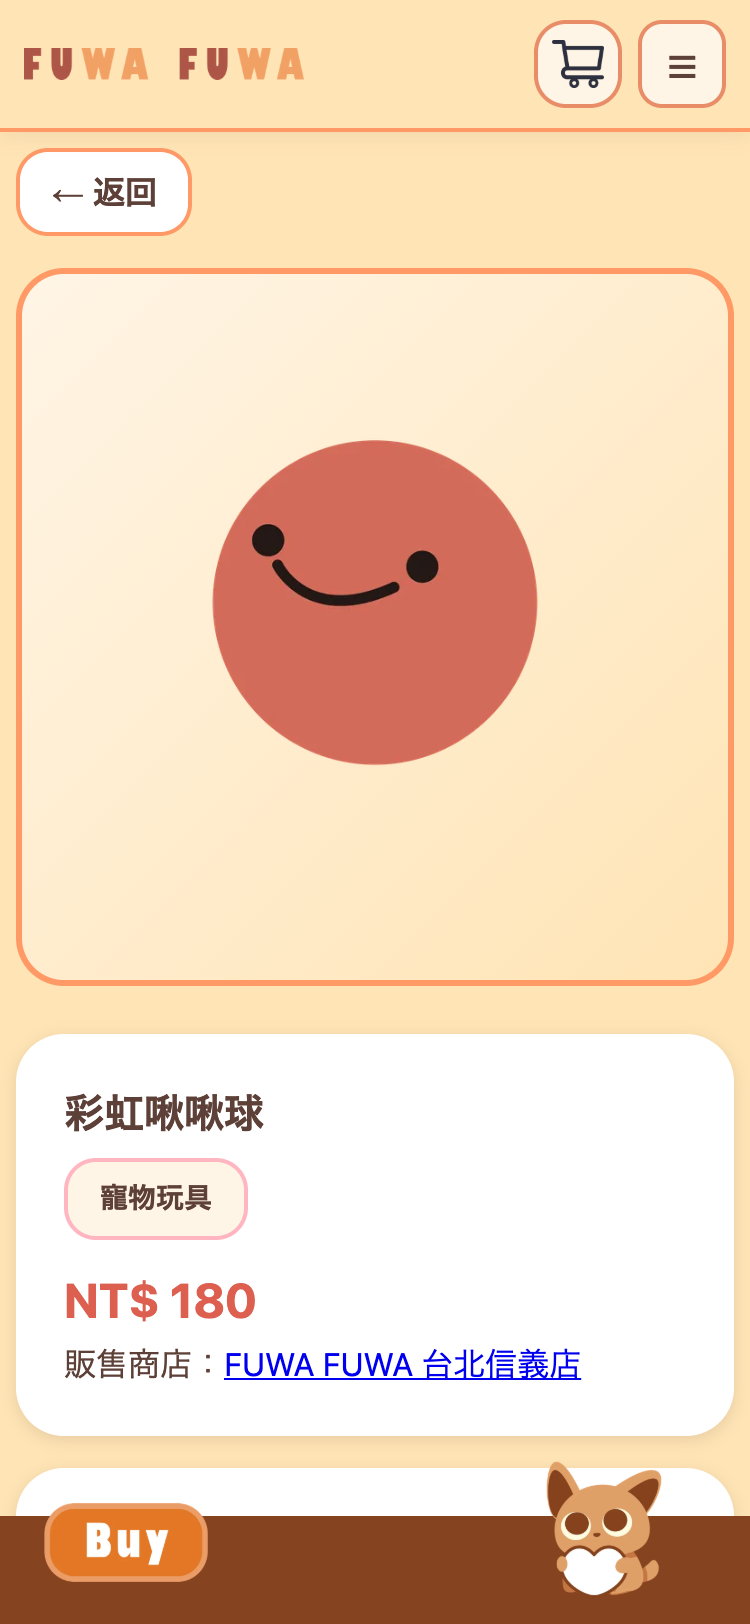
\includegraphics[width=0.36\linewidth]{img/gui_mobile_product.png}
\caption{\label{fig:gui_mobile}手機版（375 像素寬）的首頁與商品頁}
\end{figure}
